\documentclass[12pt]{article}
\usepackage{listings}
\usepackage{geometry}
\usepackage{float}
\usepackage{amsfonts}
\usepackage{amssymb}
\usepackage{caption}
\usepackage{subcaption}
\usepackage{amsmath,amssymb,amsthm}
\renewcommand{\qedsymbol}{$\blacksquare$}
 \geometry{
 a4paper,
 total={210mm,297mm},
 left=25.4mm,
 top=25.4mm,
 right = 25.4mm,
 bottom =25.4mm,
 }
\usepackage{matlab-prettifier}
\usepackage{graphicx}
\usepackage[english]{babel}
\usepackage[utf8]{inputenc}
\begin{document}
\title{Special Project 3}
\author{Jesus Javier Banuelos \\ e-mail: jesus.banuelos.951@my.csun.edu}
\maketitle
\tableofcontents
\newpage

\section{Code}
\begin{lstlisting}[
style=Matlab-editor,
basicstyle=\mlttfamily,
escapechar=`,
]
function [excel_Comp, excel_Rich]= rich_extr
clc, clear;
a=0; b=0.99; % the interval [a,b]
% Calculate the exact value of the integral
exact=asin(b)-asin(a);
S=comp_trapez(a,b,99);
Shalf=comp_trapez(a,b,198);
Stenth=comp_trapez(a,b,396);
Stenthhalf=comp_trapez(a,b,792);
Stenthhalfhalf = comp_trapez(a,b,1584);

%compute Richardson extrapolation
M=Shalf+(Shalf-S)/3;
Mhalf=Stenth+(Stenth-Shalf)/3;
Mtenth = Stenthhalf + (Stenthhalf-Stenth)/3;
Mtenthhalf = Stenthhalfhalf + (Stenthhalfhalf-Stenthhalf)/3;

% compare results: 
fprintf(1,'Trapezoidal rule, Step Size(h): %4i, S(h): %13.10f Abs Error: %13.10f \n', 0.01, S, abs(exact-S));
fprintf(1,'Trapezoidal rule, Step Size(h): %4i, S(h): %13.10f Abs Error: %13.10f Red Factor: %13.10f Order: %13.10f\n', 0.005, Shalf, abs(exact-Shalf),abs(exact-S)/abs(exact-Shalf), log(abs(exact-S)/abs(exact-Shalf))/log(2));
fprintf(1,'Trapezoidal rule, Step Size(h): %4i, S(h): %13.10f Abs Error: %13.10f Red Factor: %13.10f Order: %13.10f\n', 0.0025, Stenth, abs(exact-Stenth),abs(exact-Shalf)/abs(exact-Stenth),log(abs(exact-Shalf)/abs(exact-Stenth))/log(2));
fprintf(1,'Trapezoidal rule, Step Size(h): %4i, S(h): %13.10f Abs Error: %13.10f Red Factor: %13.10f Order: %13.10f\n', 0.00125, Stenthhalf, abs(exact-Stenthhalf), abs(exact-Stenth)/abs(exact-Stenthhalf),log(abs(exact-Stenth)/abs(exact-Stenthhalf))/log(2));
fprintf(1,'Trapezoidal rule, Step Size(h): %4i, S(h): %13.10f Abs Error: %13.10f Red Factor: %13.10f Order: %13.10f\n\n', 0.000625, Stenthhalfhalf, abs(exact-Stenthhalfhalf), abs(exact-Stenthhalf)/abs(exact-Stenthhalfhalf),log(abs(exact-Stenthhalf)/abs(exact-Stenthhalfhalf))/log(2));
fprintf(1,'Richardson extrp, Step Size(h): %4i, M(h): %13.10f Abs Error: %13.10f \n', 0.01, M, abs(exact-M));
fprintf(1,'Richardson extrp, Step Size(h): %4i, M(h): %13.10f Abs Error: %13.10f Red Factor: %13.10f Order: %13.10f\n', 0.005, Mhalf, abs(exact-Mhalf), abs(exact-M)/abs(exact-Mhalf), log(abs(exact-M)/abs(exact-Mhalf))/log(2));
fprintf(1,'Richardson extrp, Step Size(h): %4i, M(h): %13.10f Abs Error: %13.10f Red Factor: %13.10f Order: %13.10f\n', 0.0025, Mtenth, abs(exact-Mtenth), abs(exact-Mhalf)/abs(exact-Mtenth), log(abs(exact-Mhalf)/abs(exact-Mtenth))/log(2));
fprintf(1,'Richardson extrp, Step Size(h): %4i, M(h): %13.10f Abs Error: %13.10f Red Factor: %13.10f Order: %13.10f\n', 0.00125, Mtenthhalf, abs(exact-Mtenthhalf), abs(exact-Mtenth)/abs(exact-Mtenthhalf), log(abs(exact-Mtenth)/abs(exact-Mtenthhalf))/log(2));

excel_Comp = [S, abs(exact-S),0,0;...
    Shalf, abs(exact-Shalf),abs(exact-S)/abs(exact-Shalf), log(abs(exact-S)/abs(exact-Shalf))/log(2);...
    Stenth, abs(exact-Stenth),abs(exact-Shalf)/abs(exact-Stenth),log(abs(exact-Shalf)/abs(exact-Stenth))/log(2);...
    Stenthhalf, abs(exact-Stenthhalf), abs(exact-Stenth)/abs(exact-Stenthhalf),log(abs(exact-Stenth)/abs(exact-Stenthhalf))/log(2);...
    Stenthhalfhalf, abs(exact-Stenthhalfhalf), abs(exact-Stenthhalf)/abs(exact-Stenthhalfhalf),log(abs(exact-Stenthhalf)/abs(exact-Stenthhalfhalf))/log(2)];
excel_Rich = [M, abs(exact-M),0,0;...
    Mhalf, abs(exact-Mhalf), abs(exact-M)/abs(exact-Mhalf), log(abs(exact-M)/abs(exact-Mhalf))/log(2);...
    Mtenth, abs(exact-Mtenth), abs(exact-Mhalf)/abs(exact-Mtenth), log(abs(exact-Mhalf)/abs(exact-Mtenth))/log(2);...
    Mtenthhalf, abs(exact-Mtenthhalf), abs(exact-Mtenth)/abs(exact-Mtenthhalf), log(abs(exact-Mtenth)/abs(exact-Mtenthhalf))/log(2)];
function S=comp_trapez(a,b,n)
h=(b-a)/n;  %the step size
S=f(a);
for i=1:1:n-1
  S=S+2*f(a+i*h);
end
S=S+f(b);
S=(h/2)*S;

function y=f(x)
%y=sin(3*x);
y=1/sqrt(1-x.^2);
\end{lstlisting}
\section{Results of Composite Trapezoidal Rule}
\subsection{Table of Results}
\begin{figure}[H]
  \centering
  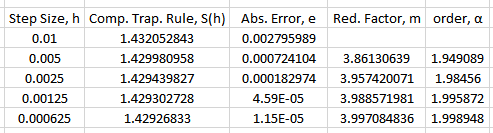
\includegraphics[width=13cm]{Comp_Trap_Rule.png}
     \caption{Composite Trapezoidal Rule}
         \label{FigVibStab}
\end{figure}
\subsection{Result Comments}
The results that I achieved do agree with the error formula given by Theorem 4.5. The error that was achieved by using the Composite Trapezoidal Rule was smaller than the biggest error we can achieve when using the error formula in Theorem 4.5.
Well when you divide h by 2 we would expect that the error would be cut down in half because the step size is being cut in half. When I ran the program with h/2 that was not the case, the error dropped about $1/4$ of its previous error. If you look at the table above the reason why I said that it would be about $1/4$ because the reduction factor was about 4 which just means that the errors are $1/4$ from each other.
\section{Development of Formula}
\begin{proof}[Derivation of Richardson Extrapolation from the Composite Trapezoidal Rule]
\begin{eqnarray}
M_1(h) = S(h) + C_2h^2+ C_3h^3+ \hdots \\
M_2(h) = S(h/2) + C_2(h/2)^2 + C_3(h/2)^3 + \hdots \\
M_3(h) = \frac{4M_2(h)-M_1(h)}{3} = \frac{1}{3}[4(S(\frac{h}{2}) + C_2(\frac{h}{2})^2 + C_3(\frac{h}{2})^3)- S(h) - C_2h^2 - C_3h^3+ \hdots] \\
= \frac{1}{3}[4S(\frac{h}{2}) + 4C_2\frac{h^2}{4} + 4C_3\frac{h^3}{8}- S(h) - C_2h^2- C_3h^3+ \hdots] \\
=\frac{1}{3}[4S(\frac{h}{2}) - S(h) + 4C_2\frac{h^2}{4}  - C_2h^2 + 4C_3\frac{h^3}{8}- C_3h^3+ \hdots]\\
=\frac{1}{3}[4S(\frac{h}{2}) - S(h) + C_2h^2  - C_2h^2 + C_3\frac{h^3}{2}- C_3h^3+ \hdots]\\
=\frac{1}{3}[4S(\frac{h}{2}) - S(h) - C_3\frac{h^3}{2}+ \hdots]\\
=\frac{1}{3}[4S(\frac{h}{2}) - S(h)]\\
=\frac{1}{3}[3S(\frac{h}{2})+S(\frac{h}{2})-S(h)]\\
M_3(h) = S(\frac{h}{2})+[\frac{S(\frac{h}{2})-S(h)}{3}]
\end{eqnarray}
\end{proof}
\section{Results of Richardson Extrapolation}
\subsection{Table of Results}
\begin{figure}[H]
  \centering
  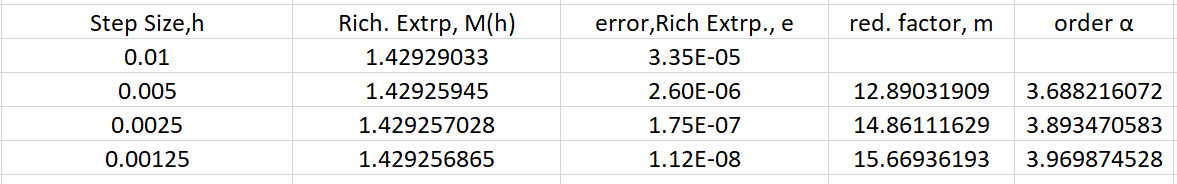
\includegraphics[width=15cm]{Rich_Extrp.png}
     \caption{Richardson Extrapolation}
         \label{FigVibStab}
\end{figure}
\subsection{Result Comments}
The error for the step size, h = 0.00125, for the Composite Trapezoidal Rule was $7.241e^{-4}$ and step size, h = 0.01, an error of $3.3476e^{-5}$ was achieved with Richardson Extrapolation. These errors are very similar with them being $1e^{-5}$ off from each other. When dealing with the step sizes mentioned before, the most efficient one between the Richardson Extrapolation and the Composite Trapezoidal Rule would have to be the Composite Trapezoidal Rule. The Richardson Extrapolation has a bigger error than the Composite Trapezoidal Rule at first, but as the step size gets smaller the error does not change much for the Composite Trapezoidal Rule. While the Richardson Extrapolation does get smaller as seen from the table from above. Thus, meaning that as we make the step size smaller the more efficient one is the Richardson Extrapolation, but the main motive was to see which of the two at specific step sizes was the more efficient one. Hence, the Composite Trapezoidal Rule is more efficient at h = $0.00125$ than the Richardson Extrapolation at h = $0.01$.
\end{document}